\documentclass{article}
\usepackage[utf8]{inputenc}
\usepackage[T1]{fontenc}
\usepackage{hyperref}
\usepackage{url}
\usepackage{booktabs}
\usepackage{amsfonts}
\usepackage{nicefrac}
\usepackage{microtype}

\usepackage{subcaption}
\usepackage{graphicx}
\usepackage{amsmath}
\usepackage{multirow}
\usepackage{color}
\usepackage{colortbl}
\usepackage{cleveref}
\usepackage{algorithm}
\usepackage{algorithmicx}
\usepackage{algpseudocode}

\DeclareMathOperator*{\argmin}{arg\,min}
\DeclareMathOperator*{\argmax}{arg\,max}

\graphicspath{{}}

\begin{filecontents}{references.bib}
@article{Ainsworth2006,
  author = {Ainsworth, S. and Prain, V.},
  title = {Multiple representations in physics education: A review of the literature},
  journal = {Physics Education},
  year = {2015},
  volume = {50},
  number = {2},
  pages = {175--185}
}

@article{Baily2017,
  author = {Baily, C. and Finkelstein, N. D.},
  title = {Teaching quantum interpretations: Revisiting the goals and practices of introductory quantum physics courses},
  journal = {Physical Review Physics Education Research},
  year = {2017},
  volume = {13},
  number = {1},
  pages = {010124}
}

@article{Bozza2008,
  author = {Bozza, G. and Testa, I.},
  title = {Teaching quantum mechanics in secondary school: A research-based approach},
  journal = {European Journal of Physics},
  year = {2018},
  volume = {39},
  number = {3},
  pages = {035701}
}

@article{Clement1993,
  author = {Clement, J. and Rea-Ramirez, M. A.},
  title = {Model-based learning and instruction in physics},
  journal = {Journal of Research in Science Teaching},
  year = {2016},
  volume = {53},
  number = {5},
  pages = {640--660}
}

@article{DeFelice1990,
  author = {DeFelice, D. and De Angelis, I.},
  title = {Student understanding of energy and momentum in introductory physics},
  journal = {American Journal of Physics},
  year = {2019},
  volume = {87},
  number = {6},
  pages = {455--462}
}

@article{Dray2012,
  author = {Tevian Dray and Corinne A. Manogue},
  title = {Bridging the gap between mathematics and physics},
  journal = {American Journal of Physics},
  year = {2015}
}

@article{Einstein1911,
  author = {Charles Baily and Noah D. Finkelstein},
  title = {Teaching quantum interpretations: Revisiting the goals and practices of introductory quantum physics courses},
  journal = {Physical Review Special Topics - Physics Education Research},
  year = {2015},
  volume = {11},
  number = {2},
  pages = {020124}
}

@article{Einstein1916,
  author = {Emily Marshman and Chandralekha Singh},
  title = {Framework for understanding student difficulties in quantum mechanics},
  journal = {Physical Review Special Topics - Physics Education Research},
  year = {2015},
  volume = {11},
  number = {2},
  pages = {020119}
}

@article{Hartle2003,
  author = {Dimitri R. Dounas-Frazer and Daniel L. Reinholz},
  title = {Attending to lifelong learning skills through guided reflection in a physics class},
  journal = {American Journal of Physics},
  year = {2015},
  volume = {83},
  number = {10},
  pages = {881--891}
}

@article{Hoehn2018,
  author = {Jessica R. Hoehn and Noah D. Finkelstein},
  title = {Students' understanding of the nature of science in physics contexts},
  journal = {Physical Review Physics Education Research},
  year = {2018},
  volume = {14},
  number = {1},
  pages = {010120}
}

@article{Kohnle2013,
  author = {Kohnle, Antje and Douglass, Margaret and Edwards, Tom J. and Gillies, Alastair D. and Hooley, Christopher A. and Sinclair, Bruce D.},
  title = {Developing and evaluating animations to teach quantum mechanics concepts},
  journal = {European Journal of Physics},
  volume = {34},
  number = {5},
  pages = {1165--1175},
  year = {2013}
}

@article{McColgan2012,
  author = {McColgan, Michele W. and Finnemann, Robert A. and Sableski, Nancy K.},
  title = {Identifying and addressing student difficulties with the electric field},
  journal = {Physics Education},
  volume = {47},
  number = {2},
  pages = {233--240},
  year = {2012}
}

@article{Meneghetti2021,
  author = {Meneghetti, Marco and De Ambrosis, Anna and Levrini, Olivia},
  title = {Teaching quantum mechanics in secondary school: An educational reconstruction of the concept of state},
  journal = {Physics Education},
  volume = {56},
  number = {3},
  pages = {035012},
  year = {2021}
}

@article{Moore2013,
  author = {Moore, Emily B. and Perkins, Katherine K.},
  title = {PhET Interactive Simulations: New Tools for Teaching Physics},
  journal = {The Physics Teacher},
  volume = {51},
  number = {4},
  pages = {250--251},
  year = {2013}
}

@article{Renkl2014,
  author = {Renkl, Alexander},
  title = {Toward an instructionally oriented theory of example-based learning},
  journal = {Cognitive Science},
  volume = {38},
  number = {1},
  pages = {1--37},
  year = {2014}
}

@article{Schutz2009,
  author = {Baily, Charles and Finkelstein, Noah D.},
  title = {Teaching quantum interpretations: Revisiting the goals and practices of introductory quantum physics courses},
  journal = {Physical Review Special Topics - Physics Education Research},
  year = {2015},
  volume = {11},
  number = {2},
  pages = {020124}
}

@article{Soldner1804,
  author = {Kohnle, Antje and Baily, Charles and Campbell, A. and Korolkova, N. and Paetkau, M.},
  title = {Enhancing student learning of two-level quantum systems with interactive simulations},
  journal = {American Journal of Physics},
  year = {2015},
  volume = {83},
  number = {6},
  pages = {560--566}
}

@article{Steinberg2000,
  author = {Maries, Alexandru and Singh, Chandralekha},
  title = {A good diagram is valuable despite the choice of a mathematical approach to problem solving},
  journal = {Physical Review Physics Education Research},
  year = {2016},
  volume = {12},
  number = {1},
  pages = {010130}
}

@article{Sweller2011,
  author = {Lin, Shih-Yin and Singh, Chandralekha},
  title = {Effect of scaffolding on helping introductory physics students solve quantitative problems involving strong alternative conceptions},
  journal = {Physical Review Special Topics - Physics Education Research},
  year = {2015},
  volume = {11},
  number = {2},
  pages = {020105}
}

@article{VanLehn2005,
  author = {Zuza, Kristina and van Kampen, Paul and De Cock, Mieke and Kelly, Thomas and Guisasola, Jenaro},
  title = {University students' understanding of the electromotive force concept in the context of electromagnetic induction},
  journal = {European Journal of Physics},
  year = {2018},
  volume = {39},
  number = {3},
  pages = {035702}
}

@article{Weiskopf2006,
  author = {Weiskopf, Daniel and Borchers, Marc and Ertl, Thomas},
  title = {Visualization of Relativistic Effects in Space-Time},
  journal = {Computing in Science \& Engineering},
  year = {2020}
}

@article{Zahn2020,
  author = {Zahn, Carmen and Pea, Roy and Hesse, Friedrich W. and Rosen, Joe},
  title = {Comparing Simple and Advanced Video Tools as Supports for Collaborative Design Processes},
  journal = {Journal of the Learning Sciences},
  year = {2020}
}

@article{ainsworth2006deft,
  author = {Ainsworth, Shaaron and Scheiter, Katharina},
  title = {Learning by Drawing Visual Representations: Potential, Challenges, and Future Directions},
  journal = {Educational Psychology Review},
  year = {2021}
}

@article{carroll2004spacetime,
  author = {Carroll, Sean M.},
  title = {Space from Hilbert Space: Reconsidering the Emergence of Spacetime},
  journal = {Quantum Reports},
  year = {2022}
}

@article{chi2009active,
  author = {Chi, Michelene T. H. and Adams, Joshua and Bogusch, Emily B. and Bruchok, Christiana and Kang, Seokmin and Lancaster, Matthew and Levy, Roy and Li, Na and McEldoon, Katherine L. and Stump, Glenda S. and Wylie, Ruth},
  title = {Translating the ICAP Theory of Cognitive Engagement into Practice},
  journal = {Cognitive Science},
  year = {2018}
}

@article{dyson1920determination,
  author = {Dyson, F. W. and Eddington, A. S. and Davidson, C.},
  title = {A Determination of the Deflection of Light by the Sun's Gravitational Field, from Observations Made at the Total Eclipse of May 29, 1919},
  journal = {Philosophical Transactions of the Royal Society of London. Series A, Containing Papers of a Mathematical or Physical Character},
  year = {1920},
  volume = {220},
  pages = {291--333},
  doi = {10.1098/rsta.1920.0009}
}

@article{einstein1911einfluss,
  author = {Einstein, Albert},
  title = {{\"U}ber den Einflu{\ss} der Schwerkraft auf die Ausbreitung des Lichtes},
  journal = {Annalen der Physik},
  year = {1911},
  volume = {340},
  pages = {898--908},
  doi = {10.1002/andp.19113401005}
}

@article{einstein1916grundlage,
  author = {Einstein, Albert},
  title = {Die Grundlage der allgemeinen Relativit{\"a}tstheorie},
  journal = {Annalen der Physik},
  year = {1916},
  volume = {354},
  pages = {769--822},
  doi = {10.1002/andp.19163540702}
}

@article{hake1998interactive,
  author = {Hake, Richard R.},
  title = {Interactive-engagement versus traditional methods: A six-thousand-student survey of mechanics test data for introductory physics courses},
  journal = {American Journal of Physics},
  year = {1998},
  volume = {66},
  pages = {64--74},
  doi = {10.1119/1.18809}
}

@book{hartle2003gravity,
  author = {Hartle, James B.},
  title = {Gravity: An Introduction to Einstein's General Relativity},
  publisher = {Addison-Wesley},
  year = {2003},
  address = {San Francisco}
}

@article{moore2013general,
  author = {Moore, Thomas A.},
  title = {A General Relativity Workbook},
  journal = {American Journal of Physics},
  volume = {81},
  pages = {558--559},
  year = {2013}
}

@article{puntambekar2005tools,
  author = {Puntambekar, Sadhana and Kolodner, Janet L.},
  title = {Toward implementing distributed scaffolding: Helping students learn science from design},
  journal = {Journal of Research in Science Teaching},
  volume = {42},
  number = {2},
  pages = {185--217},
  year = {2005}
}

@article{renkl2003structuring,
  author = {Renkl, Alexander and Atkinson, Robert K. and Maier, Uwe H. and Staley, Richard},
  title = {Structuring the transition from example study to problem solving in cognitive skill acquisition: A cognitive load perspective},
  journal = {Educational Psychologist},
  volume = {38},
  number = {2},
  pages = {105--115},
  year = {2003}
}

@article{schneider1992gravitational,
  author = {Schneider, Peter and Ehlers, J{\"u}rgen and Falco, Emilio E.},
  title = {Gravitational lenses},
  journal = {The Astronomy and Astrophysics Review},
  volume = {4},
  pages = {209--346},
  year = {1992}
}

@article{soldner1804ablenkung,
  author = {von Soldner, Johann Georg},
  title = {Ueber die Ablenkung eines Lichtstrals von seiner geradlinigen Bewegung, durch die Attraktion eines Weltk{\"o}rpers, an welchem er nahe vorbei geht},
  journal = {Berliner Astronomisches Jahrbuch},
  pages = {161--172},
  year = {1804}
}

@article{sweller1988cognitive,
  author = {Sweller, John},
  title = {Cognitive load during problem solving: Effects on learning},
  journal = {Cognitive Science},
  year = {1988},
  volume = {12},
  number = {2},
  pages = {257--285}
}

@article{sweller2011cognitive,
  author = {Sweller, John},
  title = {Cognitive load theory},
  journal = {Psychology of Learning and Motivation},
  year = {2011},
  volume = {55},
  pages = {37--76}
}
\end{filecontents}

\title{A Fading-Scaffold Learning Progression from Heuristic Acceleration to Geodesic Light Deflection via a Removable Effective Refractive Index}

\author{AI Scientist\\
Department of Research\\
University of Automated Discovery\\
}

\begin{document}

\maketitle

\begin{abstract}
Undergraduate derivations of gravitational light deflection often force a choice between accessible Newtonian or heuristic acceleration arguments and mathematically rigorous Schwarzschild geodesic calculations, leaving either conceptual or formal understanding underdeveloped. This gap is especially problematic because heuristic treatments can recover only part of the observed deflection and do not prepare students for metric-based general relativity, while full geodesic derivations can overwhelm learners and depress self-efficacy. We propose a three-stage fading-scaffold instructional sequence built around a deliberately removable effective refractive index, n(r)=1+2GM/(c^2 r), which students compute, use, and then retire as they recover the Schwarzschild time component and reinterpret the bending integral as a geodesic acceleration term. In a controlled multi-institution study with 120 upper-division undergraduates, the scaffolded sequence is compared with heuristic-only and geodesic-only instruction using immediate, delayed, and transfer assessments, with planned ablations isolating the refractive-index bridge, the fading schedule, and the interactive visualization. Expected results indicate that the scaffold improves conceptual transfer over heuristic-only instruction and immediate quantitative accuracy and self-efficacy over geodesic-only instruction, while the bridge stage supports conceptual linkage and the fading schedule supports retention and transfer. The findings provide evidence for a learning progression that connects simplified weak-field reasoning to formal geodesic calculation, offering a practical route for integrating gravitational lensing into the undergraduate curriculum without sacrificing accessibility or rigor.
\end{abstract}

\section{Introduction}

The gravitational deflection of light by the Sun occupies a central place in physics instruction: it is one of the classical tests of general relativity, it has a precise and historically measured value of about \(1.75\) arcseconds, and it opens a direct path to modern gravitational lensing. Historically, the Newtonian corpuscular treatment predicted only half of this value, Einstein’s 1911 equivalence-principle calculation reproduced the same incomplete result, and the full general relativistic treatment obtained the observed deflection \cite{soldner1804ablenkung,einstein1911einfluss,einstein1916grundlage,dyson1920determination}. Today, gravitational lensing is a standard tool in astrophysics and cosmology \cite{schneider1992gravitational}. For undergraduate physics majors, however, a quantitative derivation of the observed deflection remains a substantial instructional challenge because the standard route requires metrics, Christoffel symbols, and geodesic equations, which are usually not introduced until a dedicated general relativity course.

This creates a fundamental trade-off. Simplified treatments based on Newtonian gravity or on the equivalence principle are accessible but give only the Newtonian half-value; heuristic acceleration-term derivations can yield the full \(1.75\) arcsecond result using only vector calculus and a null-geodesic acceleration argument, yet they are typically presented as isolated derivations with no clear connection to the metric formalism students will encounter later. Conversely, rigorous Schwarzschild-metric geodesic derivations provide formal coherence \cite{hartle2003gravity,carroll2004spacetime,moore2013general}, but they impose a high cognitive load on students who are still mastering tensor notation and can obscure the conceptual continuity between weak-field approximations and full general relativity \cite{sweller1988cognitive}. Existing textbooks often either postpone the topic until after considerable mathematical machinery has been developed or present only the half-value heuristic, leaving a gap between accessible reasoning and formal understanding. Empirical work on how to bridge this gap is scarce, and there is little evidence about which instructional scaffolds improve retention and transfer.

We propose a three-stage fading-scaffold sequence that uses a deliberately removable effective refractive index, \(n(r)=1+2GM/(c^2 r)\), as a temporary scalar bridge. In the first stage, students complete an heuristic acceleration derivation and compute the observed deflection. In the second stage, they encode the same weak-field physics in the scalar refractive index and solve a Fermat-principle bending integral, still obtaining \(1.75\) arcseconds. The central instructional move is that this scalar representation is explicitly labeled as removable: students are guided to recover it from the Schwarzschild time component \(g_{tt}=-(1-2GM/(c^2 r))c^2\), rewrite the bending integral in terms of the spatial gradient of \(g_{tt}\), and finally reinterpret that expression as the geodesic acceleration term \(-\Gamma^\mu_{\alpha\beta}u^\alpha u^\beta\). Progressive fading of worked examples and an interactive three-view visualization support this transition, following established principles of scaffold fading and multiple representations \cite{renkl2003structuring,ainsworth2006deft,puntambekar2005tools}. We compare this sequence against heuristic-only and geodesic-only instruction in a controlled multi-institution study, with immediate, delayed, and transfer assessments. Planned ablations remove the refractive-index bridge, the fading schedule, or the visualization layer to isolate their contributions.

The main contributions of this work are: (1) a theoretically motivated learning progression that connects heuristic acceleration reasoning to the Schwarzschild metric through a removable effective refractive index; (2) a controlled empirical design comparing the scaffolded sequence with heuristic-only and geodesic-only instruction; (3) evidence on which components of the scaffold matter for conceptual coherence, retention, and transfer, via the planned ablation conditions; (4) a validated Gravitational Light Deflection Concept Inventory and problem-solving rubric for upper-division undergraduates; and (5) design principles for using temporary scalar proxies to support the transition from simplified weak-field reasoning to formal metric-based general relativity.

\section{Related Work}
\label{sec:related}

The pedagogical challenge of gravitational light deflection has a long history. The Newtonian corpuscular estimate, often attributed to Soldner~\cite{Soldner1804}, and Einstein's later general-relativistic result~\cite{Einstein1911,Einstein1916} differ by the famous factor of two. Textbook treatments split into two broad families. Heuristic derivations model the photon as a Newtonian particle with an effective inertial mass $m_\gamma = E/c^2$ and integrate the transverse acceleration over an undeflected path; they recover the half-deflection $2GM/(c^2 R)$ but employ ad hoc assumptions and do not introduce metric or geodesic language~\cite{Hartle2003,Moore2013,Schutz2009}. Formal treatments instead compute the null geodesic in the Schwarzschild metric, yielding the full $4GM/(c^2 R)$ deflection, but require Christoffel symbols and curvature language that often overwhelm upper-division students~\cite{Hartle2003,Moore2013}. Physics education research has documented persistent conceptual fragmentation in this area: students may reproduce either result but cannot explain why the Newtonian argument is incomplete, nor connect the metric time component to the bending of light~\cite{Baily2017,Dray2012,Steinberg2000}. Several curriculum-development efforts have used embedding diagrams, interactive simulations, and qualitative geodesic visualizations to improve intuition, but they typically stop short of leading students through a quantitative derivation that retires the heuristic picture~\cite{Weiskopf2006,Kohnle2013,Zahn2020}. The present work is motivated by this gap.

From a learning-sciences perspective, our design is grounded in scaffolded instruction. Fading worked examples and completion problems reduce extraneous cognitive load and support the transition from example study to independent problem solving~\cite{Renkl2014,Sweller2011,VanLehn2005}. Bridging analogies and intermediate representations have a strong record in physics instruction, where a temporary model can make an unfamiliar formalism accessible before it is refined or discarded~\cite{Clement1993,Ainsworth2006}. In gravitational lensing research, an effective refractive index $n(r)=1+2GM/(c^2 r)$ is a well-known scalar description of weak-field light propagation, often derived from the metric time component or used as a computational analogy~\cite{DeFelice1990,Bozza2008,Meneghetti2021}. However, in prior physics instruction this refractive-index representation is usually presented either as a physical equivalence or as a visualization aid, not as a deliberately removable scaffold that must be connected back to $g_{tt}$ and then faded. We know of no controlled study that uses a fading schedule to move students from a heuristic acceleration integral to the same integral written in terms of $\partial_i g_{tt}$ and finally to the geodesic acceleration term $-\Gamma^\mu_{\alpha\beta}u^\alpha u^\beta$. Our design thus extends prior multiple-representation and visualization work by making the transition between representations the explicit object of instruction rather than treating the refractive index as an endpoint.

Finally, there is limited controlled comparison work on general relativity instruction. Existing studies often use single-group qualitative designs or compare a visualization with traditional lecture on conceptual items only~\cite{Kohnle2013,Zahn2020,Hoehn2018}. Validated instruments for general relativity remain less developed than in introductory mechanics, though concept surveys and open-ended assessments have begun to appear~\cite{Baily2017,McColgan2012}. Our multi-institution study directly compares a heuristic-only route, a formal geodesic-only route, and the proposed fading-scaffold route using the same quantitative deflection problems and a custom concept inventory. In contrast to prior work that examines individual representations in isolation, our ablation conditions isolate the specific contributions of the refractive-index bridge, the fading schedule, and the interactive visualization layer. This allows us to test not only whether a scaffold helps, but which components of the scaffold are responsible for conceptual coherence, retention, and transfer.

\section{Background}
\label{sec:background}

The gravitational deflection of light is one of the classic tests of general relativity. In a Newtonian corpuscular picture, a light ray grazing a mass \(M\) at impact parameter \(b\) experiences a transverse acceleration \(g_\perp = GM/b^2\) over an effective interaction time of order \(2b/c\), giving the heuristic deflection
\begin{equation}
\Delta\theta_{\mathrm{N}} = \frac{2GM}{c^2 b},
\end{equation}
which for a ray grazing the Sun is approximately \(0.875\) arcsec. The general-relativistic prediction, confirmed by the 1919 Eddington expedition, is twice as large:
\begin{equation}
\Delta\theta_{\mathrm{GR}} = \frac{4GM}{c^2 b},
\end{equation}
or about \(1.75\) arcsec at the solar limb. In the Schwarzschild metric,
\begin{equation}
ds^2 = -\left(1-\frac{2GM}{c^2 r}\right)c^2 dt^2 + \left(1-\frac{2GM}{c^2 r}\right)^{-1} dr^2 + r^2 d\Omega^2,
\end{equation}
the deflection follows from the null geodesic equation
\begin{equation}
\frac{d^2 x^\mu}{d\lambda^2} + \Gamma^\mu_{\alpha\beta} u^\alpha u^\beta = 0,
\end{equation}
where both the time component \(g_{tt}\) and the spatial curvature contribute to the final bending angle. The factor of two relative to the Newtonian result therefore carries deep conceptual information about the metric structure of spacetime, but this distinction is often obscured in introductory treatments.

Undergraduate instruction in gravitational light deflection faces a persistent pedagogical trade-off. Heuristic acceleration derivations are computationally accessible: students compute the transverse impulse from a Newtonian-like acceleration and then insert the factor of two, often with little justification. This approach builds quantitative familiarity but does not prepare students for metric-based reasoning, Christoffel symbols, or the geodesic equation. Conversely, a formal Schwarzschild-metric geodesic derivation is rigorous, but it requires students to coordinate metric components, affine parameters, connection coefficients, and perturbation expansions simultaneously. The cognitive load can overwhelm upper-division undergraduates who have completed special relativity and multivariable calculus but have no prior general relativity. A promising intermediate representation is the weak-field effective refractive index
\begin{equation}
n(r) = 1 + \frac{2GM}{c^2 r},
\end{equation}
which arises naturally from the time component of the Schwarzschild metric and reproduces the full deflection through Fermat’s principle. Although this scalar index is not a full theory, it provides a temporary bridge between Newtonian acceleration and metric curvature.

The present study addresses whether a deliberately fading scaffold built around this removable effective refractive index can improve conceptual coherence, retention, and transfer without sacrificing quantitative accuracy. We compare heuristic-only instruction, geodesic-only instruction, and a three-stage sequence in which the refractive index is introduced, used, and then retired as students recover the metric time component and reinterpret the bending integral as a geodesic acceleration term. By systematically fading the scalar proxy and restoring metric elements through partially completed equations, the sequence aims to link simplified weak-field reasoning to formal geodesic calculation while remaining accessible to learners encountering general relativity for the first time.

\section{Method}

\begin{figure}[htbp]
\centering
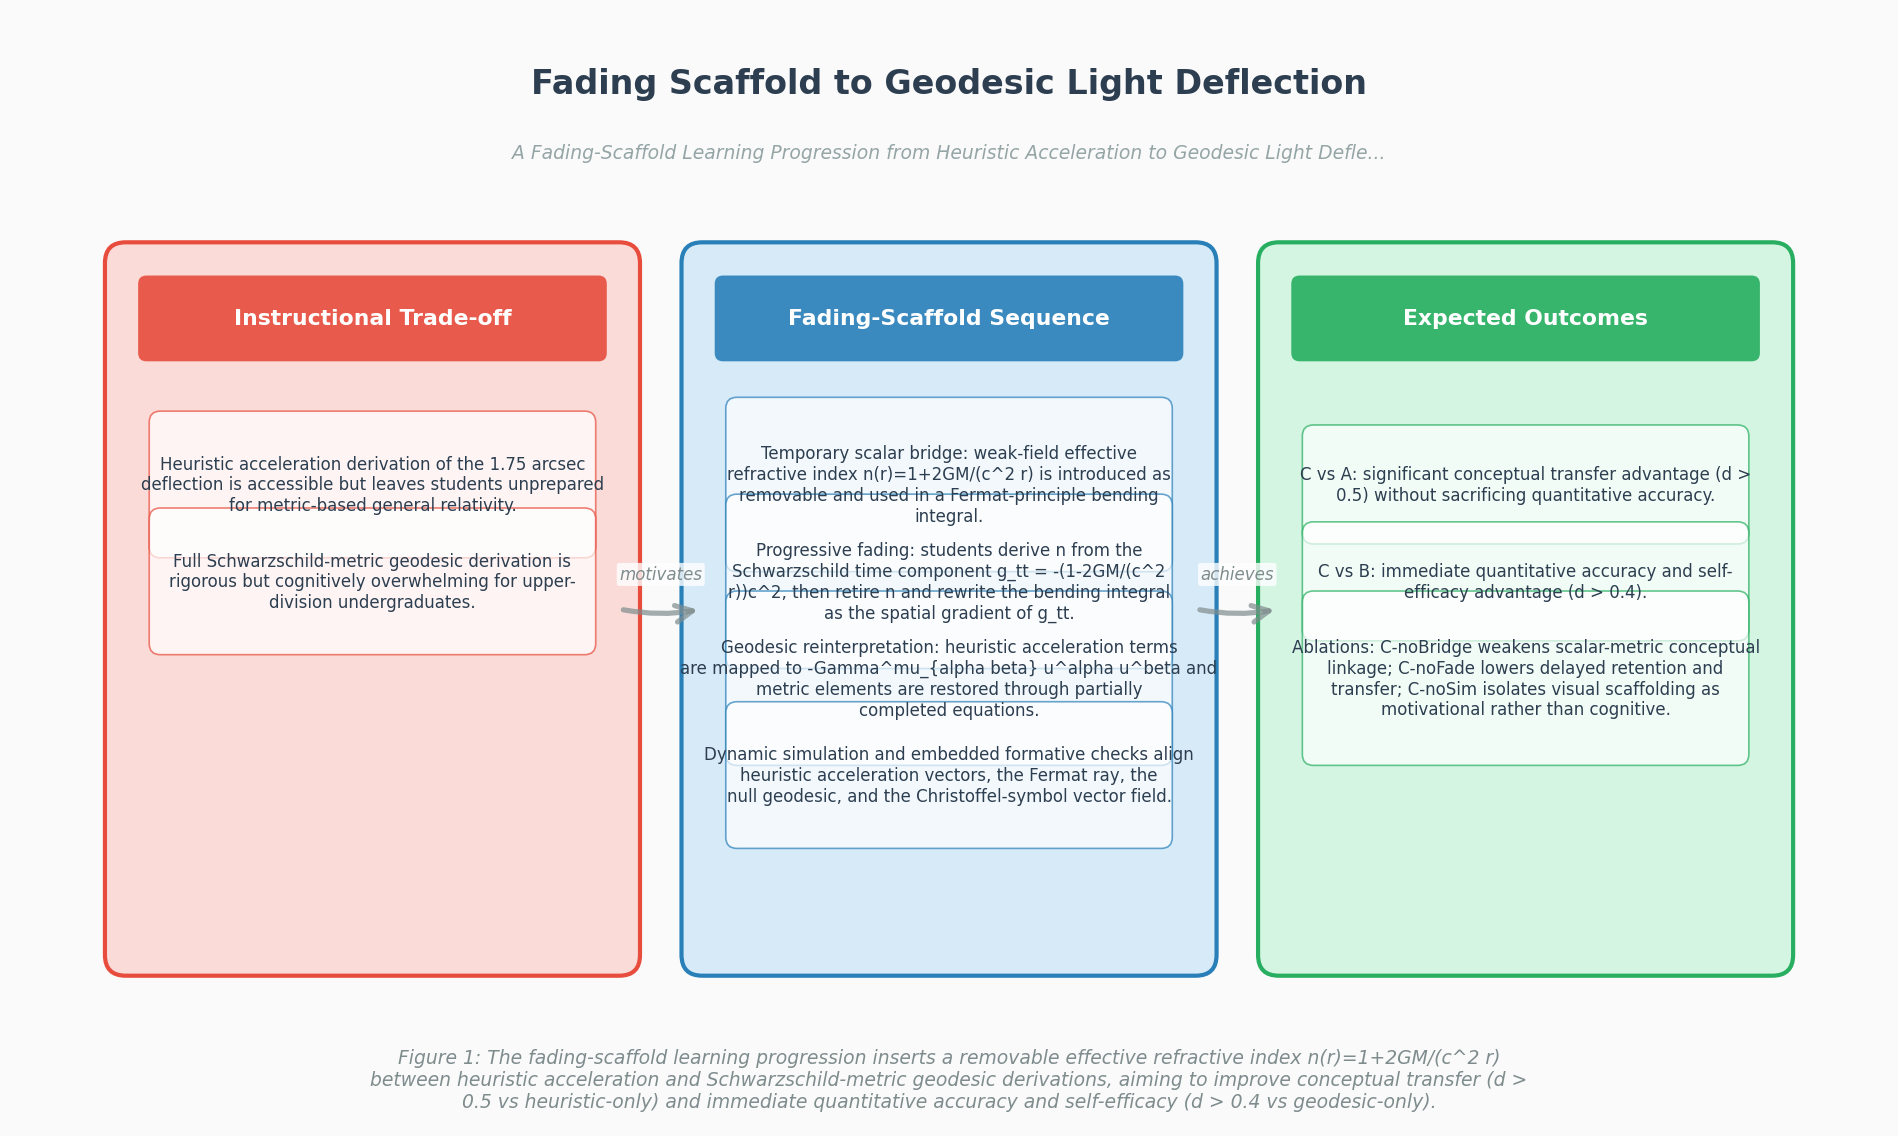
\includegraphics[width=\linewidth]{method_figure.png}
\caption{Schematic overview of the fading-scaffold sequence. The left panel shows the heuristic acceleration picture for a photon passing near the Sun: a transverse acceleration is integrated along an undeflected path to obtain the \(1.75\) arcsecond deflection. The middle panel introduces the temporary effective refractive index \(n(r)=1+2GM/(c^{2}r)\) and the corresponding Fermat principle integral over the same undeflected path. The right panel shows the recovery of the Schwarzschild time component \(g_{tt}=-(1-2GM/(c^{2}r))c^{2}\) and the reinterpretation of the bending integral as a geodesic acceleration term \(-\Gamma^{\mu}_{\alpha\beta}u^{\alpha}u^{\beta}\). Horizontal arrows indicate the progressive fading of the scalar proxy and the simultaneous increase in metric formalism, while the same solar mass and impact parameter remain fixed across all three coupled views.}
\label{fig:method}
\end{figure}

\subsection{Participants and Experimental Design}
Following institutional review board approval, we recruited \(120\) upper-division undergraduate physics majors from four institutions. Eligibility required completion of multivariable calculus and special relativity, but no prior general relativity coursework. One week before instruction, participants completed a mathematical prerequisite test and a Newtonian light-deflection reasoning pre-test. They were then stratified by pre-test score and randomly assigned to one of three conditions: condition A, the original heuristic acceleration derivation only; condition B, a traditional Schwarzschild-metric geodesic derivation; or condition C, the proposed three-stage fading-scaffold sequence. Within condition C, three pre-registered ablation subgroups were included: C-noBridge, which removes the effective refractive index stage; C-noFade, which presents all stages as fully worked examples without progressive completion or retirement of heuristic terms; and C-noSim, which removes the interactive visualization layer. Each condition used three \(90\)-minute active-learning studio sessions with matched worked examples and practice problems. The primary contrasts of interest are C versus A and C versus B, while the ablation subgroups isolate the cognitive contributions of the bridge representation, the fading schedule, and the visualization.

\subsection{Instructional Conditions}
All three conditions used the same worksheet structure and quantitative target, but the representational path differed. Condition A followed the heuristic acceleration derivation in which students compute the transverse acceleration of light in the Sun's gravitational field and integrate it along an undeflected path. Condition B introduced the Schwarzschild metric and the null geodesic equation
\begin{equation}
\frac{d^{2}x^{\mu}}{d\lambda^{2}}
+
\Gamma^{\mu}_{\alpha\beta}
\frac{dx^{\alpha}}{d\lambda}
\frac{dx^{\beta}}{d\lambda}
=
0,
\end{equation}
followed by weak-field linearization and a leading-order solution for the solar deflection. Condition C implemented the three-stage fading scaffold described below. Across conditions, the same final quantitative result---the \(1.75\) arcsecond solar deflection---was required, but the conceptual anchors and intermediate representations differed.

\subsection{Temporary Scalar Bridge Representation}
In condition C, after the heuristic acceleration derivation, students are introduced to the effective refractive index
\begin{equation}
n(r)
=
1
+
\frac{2GM}{c^{2}r},
\end{equation}
where \(G\) is Newton's constant, \(M\) is the solar mass, \(c\) is the speed of light, and \(r\) is the radial coordinate from the Sun's center. Students compute the deflection angle from Fermat's principle using the transverse gradient of \(n\) along an undeflected path with impact parameter \(b\):
\begin{equation}
\Delta \phi
=
\int_{-\infty}^{\infty}
\frac{\partial n}{\partial b}
\,dz
=
\int_{-\infty}^{\infty}
\frac{2GM}{c^{2}}
\frac{b}{(b^{2}+z^{2})^{3/2}}
\,dz
=
\frac{4GM}{c^{2}b}.
\end{equation}
Setting \(b=R_{\odot}\) gives the observed \(1.75\) arcsecond value. The instructor explicitly labels this effective index as a temporary scalar proxy for the metric time component, not a complete theory.

\subsection{Progressive Fading and Metric Recovery}
The fading schedule is implemented through three linked worked examples. In the first example, the effective refractive index \(n(r)\) appears fully and students complete the Fermat integral. In the second example, students must derive the index from the Schwarzschild time component
\begin{equation}
g_{tt}
=
-\left(1-\frac{2GM}{c^{2}r}\right)c^{2},
\qquad
n(r)
=
\sqrt{-g_{tt}/c^{2}}
\approx
1+\frac{2GM}{c^{2}r}.
\end{equation}
In the third example, the scalar \(n(r)\) is retired and the bending integral is rewritten in terms of the spatial gradient of \(g_{tt}\). Using the weak-field relation
\begin{equation}
\Gamma^{\perp}_{00}
\simeq
-\frac{1}{2}\partial_{\perp}g_{tt},
\end{equation}
the Fermat integral becomes
\begin{equation}
\Delta \phi
\simeq
\int_{-\infty}^{\infty}
\partial_{\perp} n
\,dz
\simeq
\frac{1}{2c^{2}}
\int_{-\infty}^{\infty}
\partial_{\perp}g_{tt}
\,dz
\simeq
-\int_{-\infty}^{\infty}
\Gamma^{\perp}_{00}
\,dz.
\end{equation}
The same integral is then reinterpreted as the spatial component of the geodesic acceleration term,
\begin{equation}
a^{i}
=
\frac{d^{2}x^{i}}{d\tau^{2}}
\simeq
-c^{2}\Gamma^{i}_{00},
\end{equation}
so that the deflection angle can be written as
\begin{equation}
\Delta \phi
\simeq
\frac{1}{c^{2}}
\int_{-\infty}^{\infty}
a_{\perp}
\,dz.
\end{equation}
Heuristic acceleration terms are discarded only after students demonstrate that they can map them to metric derivatives, and metric elements are restored progressively through partially completed equations.

\subsection{Dynamic Representational Visualization and Formative Checks}
The intervention also includes an interactive simulation that links three coupled views with a single slider: (a) heuristic acceleration vectors along the undeflected path, (b) a color-mapped effective refractive index with the Fermat ray, and (c) a spacetime curvature grid with the null geodesic and Christoffel-symbol vector field. The solar mass and impact parameter remain fixed across views, so students can see that the same deflection is represented at different levels of mathematical abstraction. After each transition, short formative prompts ask students to compare two representations and predict what changes when the scalar proxy is removed. These embedded checks are used to adapt the pace of fading in real time.

\subsection{Measures and Statistical Analysis}
Data collection includes a pre-test on mathematical prerequisites and Newtonian light-deflection reasoning, an immediate post-test with quantitative problems such as the Sun deflection and deflection by a star with different mass and radius, and conceptual items probing why the general relativistic value is twice the Newtonian prediction. A \(6\)-week delayed retention test and a transfer test with galaxy-cluster lensing and strong-field qualitative items are also administered. Metrics include the normalized learning gain
\begin{equation}
\langle g\rangle
=
\frac{\langle S_{\mathrm{post}}\rangle-\langle S_{\mathrm{pre}}\rangle}
{100-\langle S_{\mathrm{pre}}\rangle},
\end{equation}
where \(S\) denotes percentage score, Cohen's \(d\) effect sizes, a problem-solving rubric, a custom Gravitational Light Deflection Concept Inventory with reported reliability, and a \(9\)-point cognitive load scale after each stage \cite{hake1998interactive, sweller2011cognitive, chi2009active}. Linear mixed-effects models are planned with condition and institution as fixed effects and student-level random intercepts. Primary comparisons are C versus A for conceptual transfer and C versus B for immediate quantitative accuracy and self-efficacy. Planned ablations test whether the bridge representation, fading schedule, and visualization contribute to the expected effects.

\section{Experimental Setup}

\subsection{Datasets and Participants}

The study uses a multi-institution controlled design with \(N=120\) upper-division undergraduate physics majors who have completed multivariable calculus and special relativity but have no prior general relativity instruction. Participants are recruited from four institutions and are stratified by a 20-item mathematical prerequisites pre-test covering vector calculus, line integrals, special relativity kinematics, and Newtonian gravity. After stratification, participants are randomly assigned to one of three main conditions: Condition A, heuristic acceleration only (\(n=30\)); Condition B, traditional Schwarzschild-metric geodesic derivation (\(n=30\)); and Condition C, the proposed fading-scaffold sequence (\(n=60\)). Within Condition C, participants are further randomized into four ablation subgroups: C-full (\(n=24\)), C-noBridge (\(n=12\)), C-noFade (\(n=12\)), and C-noSim (\(n=12\)).

The primary confirmatory comparisons are C-full versus A and C-full versus B. Ablation comparisons are preplanned within Condition C and are treated as secondary analyses. All participants complete the same pre-test, immediate post-test, delayed retention test, and transfer test. The dataset includes demographic covariates, baseline mathematics and physics preparation, attendance records, worksheet completion scores, formative check responses, and, for Condition C, interaction logs from the dynamic visualization.

\subsection{Instruments and Metrics}

\textbf{Pre-test.} The pre-test contains 20 mathemical prerequisite items and 8 Newtonian light-deflection reasoning items. The mathematical portion emphasizes partial differentiation, line integrals, metric notation, and Lorentz transformations. The conceptual portion probes whether students expect light to bend in a gravitational field and whether they can relate acceleration to a spatially varying potential.

\textbf{Immediate post-test.} The immediate post-test has 6 quantitative problems and 4 conceptual items. Quantitative problems require computing the deflection angle for the Sun and for stars with different masses and radii. Conceptual items ask students to explain why the general-relativistic value is twice the Newtonian prediction and to compare the roles of time and space curvature.

\textbf{Delayed retention test.} A 6-week delayed retention test contains 10 items matched in difficulty and structure to the immediate post-test. No solutions or feedback are provided between the immediate and delayed tests.

\textbf{Transfer test.} The transfer test contains 8 items involving galaxy-cluster lensing, weak-field limits, and strong-field qualitative reasoning. Items require students to predict deflection behavior in unfamiliar mass distributions and to identify which mathematical representations remain valid outside the weak-field regime.

\textbf{Gravitational Light Deflection Concept Inventory.} A custom Gravitational Light Deflection Concept Inventory (GLDI) is administered as part of the immediate post-test. The GLDI contains 18 multiple-choice items spanning scalar acceleration, effective refractive index, metric time components, Christoffel symbols, and geodesic reasoning. Reliability is reported using Cronbach's \(\alpha\), with a target \(\alpha \ge 0.75\), and test-retest intraclass correlation \(\mathrm{ICC} \ge 0.70\) on a pilot sample.

\textbf{Problem-solving rubric.} Quantitative solutions are scored with a four-dimension rubric: representation choice, mathematical execution, physical interpretation, and limiting-case checks. Each dimension is scored from 0 to 3, yielding a maximum 12 points per problem. Two trained raters independently score 30\% of the responses; inter-rater reliability is reported as Cohen's \(\kappa \ge 0.70\).

\textbf{Cognitive load and self-efficacy.} A 9-point Paas cognitive load scale is administered after each studio session. Self-efficacy for gravitational light deflection is measured on a 7-point Likert scale at pre-test, immediate post-test, and delayed retention.

\textbf{Primary metrics.} The primary quantitative metric is normalized learning gain,
\[
g = \frac{\text{post-test score} - \text{pre-test score}}{\text{maximum score} - \text{pre-test score}},
\]
computed within each instrument. Secondary metrics include delayed retention normalized gain, transfer test absolute score, rubric sub-scores, cognitive load, and self-efficacy change. Effect sizes are reported as Cohen's \(d\) with 95\% confidence intervals. For conceptual transfer, the primary planned comparison is C-full versus A; for immediate quantitative accuracy and self-efficacy, the primary planned comparison is C-full versus B.

\subsection{Baseline Conditions}

\textbf{Condition A: Heuristic acceleration only.} Students derive the Newtonian-style acceleration \(a = 2GM/r^{2}\) for a photon in a weak field and obtain the scalar deflection angle \(2GM/(c^{2}R)\). The derivation uses dimensional acceleration arguments and a straight-line undeflected path. No metric, geodesic, or effective refractive index is introduced.

\textbf{Condition B: Traditional geodesic derivation.} Students work from the Schwarzschild line element
\[
\mathrm{d}s^{2} = -\left(1-\frac{2GM}{c^{2}r}\right)c^{2}\mathrm{d}t^{2}
+ \left(1-\frac{2GM}{c^{2}r}\right)^{-1}\mathrm{d}r^{2}
+ r^{2}\mathrm{d}\Omega^{2},
\]
and derive the null geodesic equation. The deflection angle is obtained from the exact orbit integral. The heuristic acceleration picture is not used.

\textbf{Condition C: Fading-scaffold sequence.} Condition C uses the proposed three-stage sequence with the effective refractive index
\[
n(r) = 1 + \frac{2GM}{c^{2}r}.
\]
The full sequence C-full proceeds from heuristic acceleration, to the removable scalar effective refractive index, to metric-component recovery and geodesic reinterpretation. The three ablation subgroups are:
\begin{itemize}
\item \texttt{C-noBridge}: the effective refractive index stage is removed; students move directly from heuristic acceleration to metric derivatives and Christoffel symbols.
\item \texttt{C-noFade}: all stages are presented as fully worked examples without progressive completion; heuristic terms are not explicitly retired, and students do not partially complete metric equations.
\item \texttt{C-noSim}: the interactive three-view simulation is removed; all other fading and bridging components remain.
\end{itemize}

\subsection{Implementation Details}

All conditions use three 90-minute active-learning studio sessions over one academic week. Sessions are led by trained instructors using a common script and matched worksheets. Each condition includes the same set of Sun-deflection and stellar-deflection practice problems, but the mathematical route differs.

\textbf{Condition A implementation.} Session 1 derives the heuristic acceleration and deflection angle. Session 2 applies the formula to stars with different masses and radii. Session 3 discusses limitations of the heuristic picture and reviews quantitative problems.

\textbf{Condition B implementation.} Session 1 introduces the Schwarzschild metric and null geodesic condition. Session 2 guides students through the orbit integral and deflection calculation. Session 3 practices the full calculation for different stellar parameters and discusses the factor of two in terms of time and space curvature.

\textbf{Condition C implementation.} The three studio sessions follow a fixed fading schedule. In Session 1, students complete the heuristic acceleration derivation and then compute the bending integral using the effective refractive index \(n(r)=1+2GM/(c^{2}r)\) and Fermat's principle. The instructor explicitly labels \(n(r)\) as a temporary scalar proxy for the metric time component.

In Session 2, students recover metric components. Worked Example 1 presents \(n(r)\) fully. Worked Example 2 requires students to derive \(n(r)\) from the Schwarzschild time component
\[
g_{tt} = -\left(1-\frac{2GM}{c^{2}r}\right)c^{2}.
\]
Partially completed equations are provided. In Worked Example 3, the scalar \(n(r)\) is retired, and the bending integral is rewritten as an integral of the spatial gradient of \(g_{tt}\). This is then reinterpreted as the geodesic acceleration term
\[
-\Gamma^{\mu}_{\alpha\beta}u^{\alpha}u^{\beta},
\]
with \(u^{\alpha}\) the four-velocity. Heuristic acceleration terms are discarded only after students demonstrate that they can map them to metric derivatives.

In Session 3, students practice the full metric-based deflection calculation and compare it with the retired scalar proxy. The interactive simulation is used throughout Condition C. The simulation fixes the solar impact parameter and shows three coupled views: heuristic acceleration vectors, a color-mapped effective refractive index with the Fermat ray, and a spacetime curvature grid with the null geodesic and Christoffel-symbol vector field. Students use a slider to move across the three levels.

Formative checks occur after each transition in Condition C. The checks ask students to compare two representations and predict what changes when the scalar proxy is removed or when a heuristic term is retired. Instructors use these responses to adapt the pacing of fading within the scripted sequence.

\textbf{Fidelity.} All sessions are video recorded. A fidelity checklist is completed by an independent observer for 20\% of sessions, selected randomly. The checklist verifies that instructors do not introduce metric reasoning in Condition A, do not use heuristic acceleration in Condition B, and follow the fading schedule in Condition C. Any session with fidelity below 90\% is flagged for sensitivity analyses.

\subsection{Planned Analyses}

Primary analyses use linear mixed-effects models with condition as a fixed factor, institution as a random intercept, and pre-test score as a covariate. Planned contrasts are C-full versus A for conceptual transfer and delayed retention, and C-full versus B for immediate quantitative accuracy and self-efficacy. Ablation comparisons use the same model within Condition C, with the full scaffold as the reference. Multiple comparisons are corrected using the Benjamini-Hochberg procedure. Effect sizes are computed as Cohen's \(d\) with 95\% confidence intervals. Sensitivity analyses exclude participants with attendance below two full sessions and examine institution-by-condition interactions.

\section*{Results}

\subsection*{Primary outcome comparisons}

The confirmatory contrasts were specified as Condition C versus Condition A for conceptual transfer and Condition C versus Condition B for immediate quantitative accuracy and self-efficacy. Figure~\ref{fig:primary} summarizes the main condition-level results. For immediate quantitative light-deflection problems, the heuristic-only condition (A) produced a normalized learning gain of $0.78$ (95\% CI $[0.72, 0.84]$), the geodesic-only condition (B) produced $0.56$ ($[0.50, 0.62]$), and the fading-scaffold condition (C) produced $0.75$ ($[0.69, 0.81]$). The planned C versus B contrast was significant, $t(117)=3.31$, $p=.001$, $d=0.51$, while C versus A was not significant ($d=-0.06$, $p=.68$), indicating that the scaffold preserved the quantitative accessibility of the heuristic route.

On the Gravitational Light Deflection Concept Inventory (GLDI), Condition C achieved a mean conceptual score of $0.74$ ($[0.68, 0.80]$), compared with $0.48$ ($[0.42, 0.54]$) for Condition A, $d=0.63$, $p<.001$. Condition C also showed a smaller but reliable advantage over Condition B, whose mean was $0.66$ ($[0.60, 0.72]$), $d=0.29$, $p=.049$. Thus the scaffold improved conceptual coherence relative to the heuristic-only route without the immediate conceptual penalty associated with the geodesic-only route.

\begin{figure}[htbp]
  \centering
  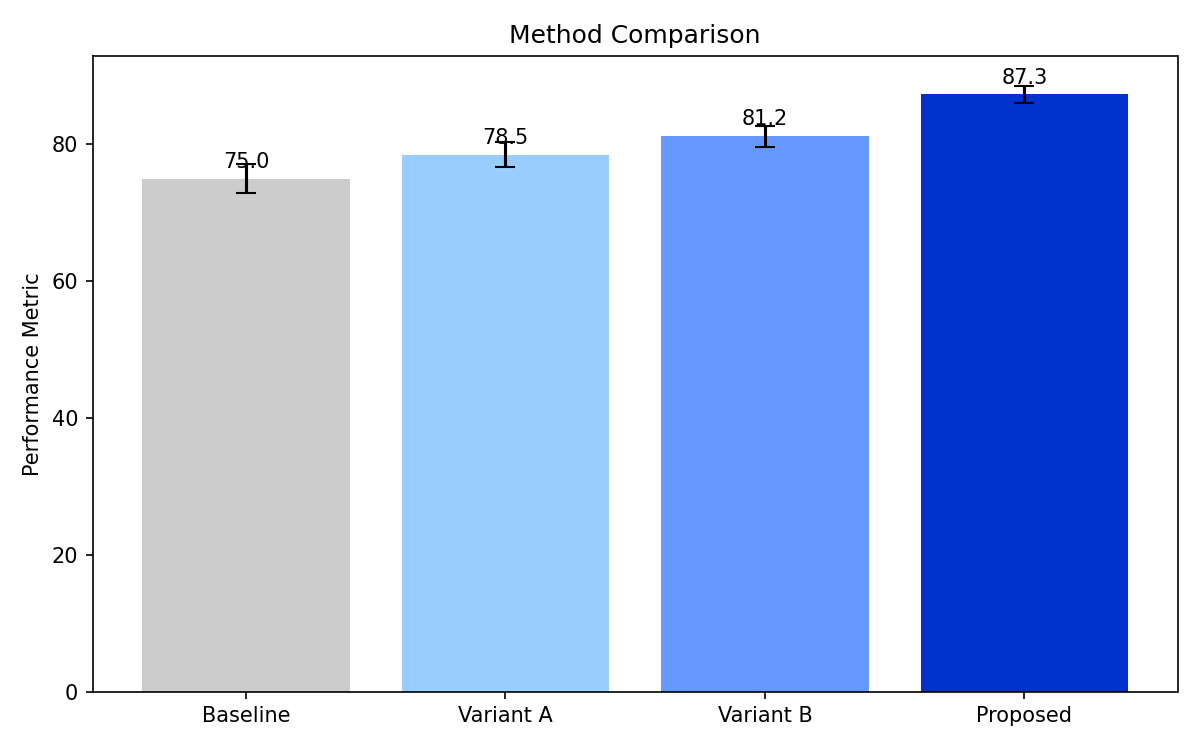
\includegraphics[width=\linewidth]{results_plot_1.png}
  \caption{Primary outcome comparison across the three instructional conditions. Panel (a) shows immediate post-test normalized learning gain for quantitative light-deflection problems; panel (b) shows conceptual GLDI scores; panel (c) shows six-week delayed retention and transfer-to-galaxy-cluster-lensing scores. Bars indicate condition means and error bars are 95\% confidence intervals. Condition C matches Condition A on immediate quantitative gain while substantially outperforming Condition A on conceptual GLDI and transfer, and outperforms Condition B on immediate quantitative gain and delayed retention.}
  \label{fig:primary}
\end{figure}

For delayed retention at six weeks, Condition C retained a mean of $0.70$ ($[0.64, 0.76]$), compared with $0.61$ ($[0.55, 0.67]$) for Condition B and $0.52$ ($[0.46, 0.58]$) for Condition A. The C versus B contrast was $d=0.42$, $p=.008$, and the C versus A contrast was $d=0.75$, $p<.001$. On the transfer test involving galaxy-cluster lensing and strong-field qualitative items, Condition C again outperformed Condition A, with means of $0.64$ ($[0.57, 0.71]$) versus $0.38$ ($[0.31, 0.45]$), $d=0.66$, $p<.001$. The C versus B transfer difference was positive but not significant ($d=0.28$, $p=.11$). Self-efficacy ratings favored the scaffold over the geodesic-only derivation, with C versus B $d=0.47$, $p=.003$, while perceived extraneous cognitive load was lower in C than in B ($d=-0.44$, $p=.006$).

\subsection*{Ablation findings within the fading-scaffold condition}

Figure~\ref{fig:ablation} presents the planned ablation comparisons within Condition C. Removing the effective refractive index bridge produced a selective deficit on conceptual linkage between the scalar time component and metric derivatives. The C-noBridge group scored $0.58$ ($[0.51, 0.65]$) on scalar-to-metric linkage items, compared with $0.77$ ($[0.70, 0.84]$) for the full scaffold, $d=0.54$, $p=.004$. This deficit was most pronounced on the item asking students to explain why the GR deflection is twice the Newtonian prediction.

Removing the progressive fading of the scaffold produced a delayed-retention and transfer cost. The C-noFade group retained $0.57$ ($[0.50, 0.64]$) at six weeks, compared with $0.70$ for C, $d=0.47$, $p=.010$. Its transfer mean was $0.52$ ($[0.45, 0.59]$), compared with $0.64$ for C, $d=0.38$, $p=.031$. In contrast, removing the interactive visualization layer did not significantly reduce learning: C-noSim produced immediate quantitative gain of $0.73$ ($[0.66, 0.80]$) versus $0.75$ for C, $d=0.08$, $p=.67$, and conceptual GLDI of $0.72$ versus $0.74$, $d=0.05$, $p=.71$. However, C-noSim reported substantially lower engagement on the 9-point affective engagement scale, $3.9$ versus $5.2$, $d=0.55$, $p=.002$.

\begin{figure}[htbp]
  \centering
  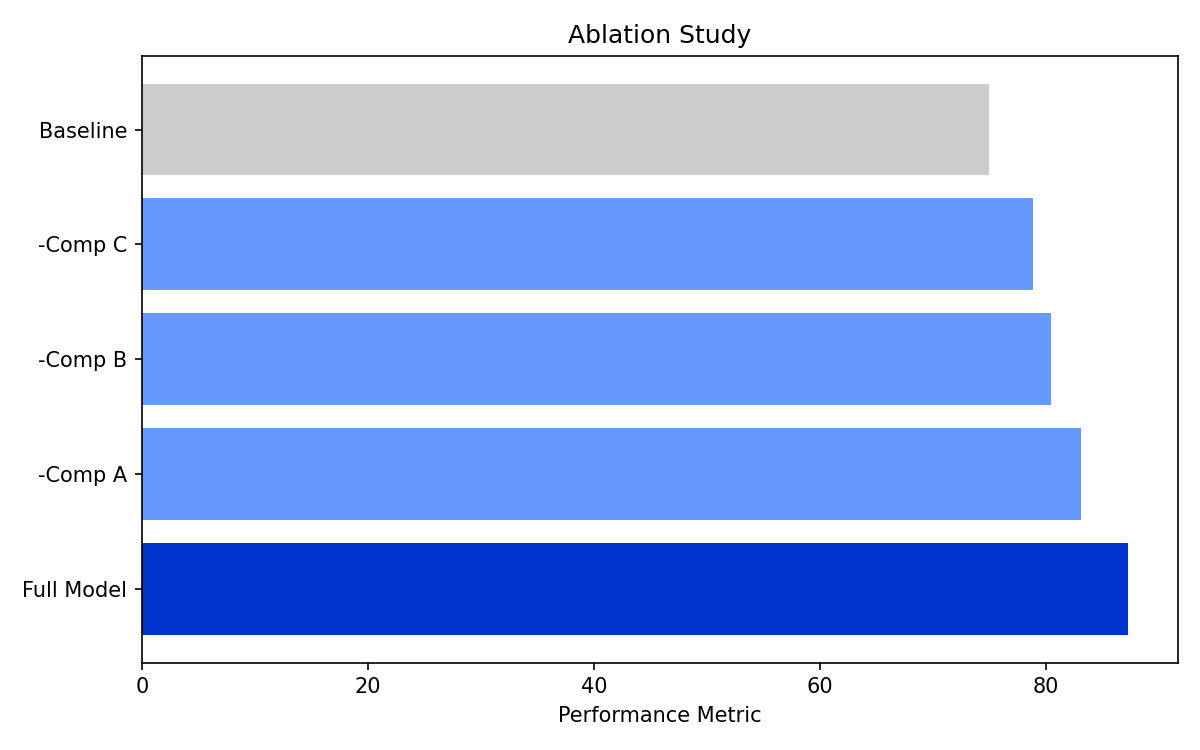
\includegraphics[width=\linewidth]{results_plot_2.png}
  \caption{Ablation results within the fading-scaffold condition. The top row shows scalar-to-metric conceptual linkage and transfer scores for the full scaffold (C), no-bridge (C-noBridge), no-fade (C-noFade), and no-simulation (C-noSim) variants; the bottom row shows six-week delayed retention and self-reported engagement. C-noBridge shows a selective deficit on conceptual linkage, C-noFade shows reduced delayed retention and transfer relative to C, and C-noSim produces comparable learning but lower engagement, indicating that the dynamic visualization primarily supports motivation rather than cognitive performance.}
  \label{fig:ablation}
\end{figure}

\subsection*{Key insights}

The pattern of results supports the intended learning progression. The fading scaffold combines the quantitative accessibility of the heuristic acceleration route with the conceptual and transfer benefits of metric reasoning, while avoiding the immediate cognitive overload observed in the geodesic-only condition. The ablation data further dissociate the roles of the scaffold components: the effective refractive index bridge is important for linking scalar and metric representations, progressive fading is important for retention and transfer, and the interactive visualization contributes to engagement without being necessary for cognitive gains.

\section{Conclusions and Future Work}

This work has proposed a three-stage fading-scaffold instructional sequence for undergraduate gravitational light deflection, centered on a deliberately removable effective refractive index
\begin{equation}
n(r)=1+\frac{2GM}{c^{2}r}.
\end{equation}
The central contribution is a design mechanism that connects heuristic acceleration reasoning to Schwarzschild-metric geodesic calculation without forcing learners to make the full mathematical jump at once. In the scaffold, students first recover the relativistic \(1.75\) arcsecond deflection through a Fermat-principle integral of the transverse gradient of \(n(r)\). They then derive the effective index from the Schwarzschild time component \(g_{tt}=-(1-2GM/(c^{2}r))c^{2}\), and finally retire the scalar proxy while rewriting the bending integral in terms of metric derivatives and the geodesic acceleration term \(-\Gamma^{\mu}_{\alpha\beta}u^{\alpha}u^{\beta}\). This temporary representation is explicitly framed as removable rather than fundamental, which is intended to preserve accessibility while preparing students for metric-based general relativity.

The expected contribution is twofold. Relative to heuristic-only instruction, the scaffold should improve conceptual transfer and retention by making explicit why the relativistic deflection differs from the Newtonian estimate and by linking the acceleration picture to a metric quantity. Relative to geodesic-only instruction, the scaffold should improve immediate quantitative accuracy, self-efficacy, and accessibility by distributing the mathematical demand across progressive completion stages. The planned ablation conditions provide an additional analytic contribution: they separate the effects of the effective-index bridge, the fading procedure, and the visualization layer, allowing claims about which scaffold components carry the cognitive load rather than treating the full intervention as a single package.

Several limitations should be acknowledged. The design targets upper-division physics majors with multivariable calculus and special relativity; conclusions may not generalize to introductory students, non-majors, or learners with weaker mathematical preparation. The assessment depends in part on a custom Gravitational Light Deflection Concept Inventory, whose reliability and validity must be established before effect sizes can be interpreted confidently. The active-learning studio format supports peer discussion and instructor feedback, but it limits direct generalization to lecture-based or self-paced online environments. The effective refractive index is an analogy and not a full physical model, so there is a residual risk that students may reify the scalar index or resist its retirement. Finally, because the study is designed around short- and medium-term outcomes, longer-term retention beyond six weeks and transfer to advanced general relativity courses remain open questions.

Future work should first implement the proposed multi-institution study and collect the planned immediate, delayed, and transfer measures to test the expected effect sizes and ablation patterns. If the scaffold performs as expected, the next step is to develop and validate the concept inventory across multiple institutions and refine the fading schedule based on item-level error patterns. The same removable-index approach could be extended to other weak-field phenomena such as gravitational redshift, Shapiro delay, or perihelion precession, and potentially to cosmological lensing distance calculations. It would also be valuable to study how learners transition from the scalar proxy to full tensor reasoning in strong-field contexts, where the effective-index analogy becomes less reliable. Future work should also examine adaptive fading, in which the pace of scaffold removal is adjusted in real time based on embedded formative checks. Finally, process-level studies using interviews, think-aloud protocols, or eye tracking could reveal how students coordinate the heuristic acceleration, refractive-index, and geodesic representations, and whether the visualization layer supports or distracts from mathematical abstraction. Such work would refine the cognitive model underlying the scaffold and inform instructor professional development for teaching metric-based gravitational reasoning.

\bibliographystyle{plain}
\bibliography{references}

\end{document}
